\chapter{Culvert functionality}

\section{Field of application}

\subsection{Flood control area in the Scheldt estuary}
Flood Control Areas (FCA) together with a Controlled Reduced Tide (CRT) system
are implemented in the Scheldt estuary to reduce the risk of flooding.
The former is defined by an area specifically located in the regions where
the bottom elevation is lower than the mean tide elevation.
This area is surrounded by an outer higher dyke and in the interface with the river,
it has a lower dyke that allows the flow to overtop the structure during storm surges.
The CRT is based on the construction of inlet and outlet sluices that control the
flow between the river and the floodplain depending on the water levels on both
sides (Figure \ref{fig:culvert_fig1}) (Teles, 2014).

\begin{figure}[H]
\begin{center}
  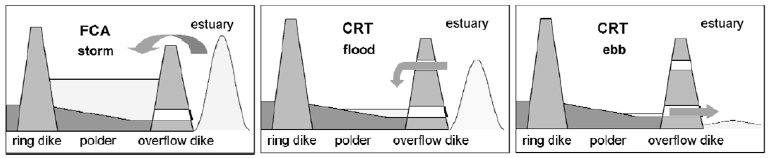
\includegraphics[width=0.95\textwidth]{culvert_fig1.png}
\end{center}
\caption{Water movements between the FCA and river without
CRT (on the left) and with CRT (on the middle and right pannels).
(Source: De Mulder et al. (2013)).}
\label{fig:culvert_fig1}
\end{figure}

The incorporation of these structures in numerical models is essential
to better predict and describe the flow hydrodynamics going to and
coming from these areas. The inlet and outlet sluices act like a weir
when they are not fully submerged and when water levels rise above the
inlet ceiling pressurised flow formulae are used.
The calibration of the head loss coefficients for the inlet and outlet sluices
was done comparing model results with measured water levels and discharges of
one specific CFA/CRT, called Lippenbroek.
Later these values were validated using the measurements from the CFA/CRT Bergenmeersen.
The coefficients found in this calibration/validation exercise are used for all the
other inlet and outlet sluices for the other FCA, FCA/CRT areas in the 3D model.

\section{Flow through a culvert: theoretical background}

A number of studies regarding the description of flows through the culverts
refer to Bodhaine's work (1968).
Bodhaine categorized the flow through a culvert into six types, and for each type
the discharge is calculated in a different way.
The equations are deduced from the continuity and energy equations between the approach
section (see Figure \ref{fig:culvert_fig2}) and the exit (downstream) section of the culvert.
The type of flow depends on whether the culvert flows full and whether the flow is controlled
by the entrance or exit part of the culvert. Figure \ref{fig:culvert_fig2}
shows a sketch for culvert flow definition.

\begin{figure}[H]
\begin{center}
  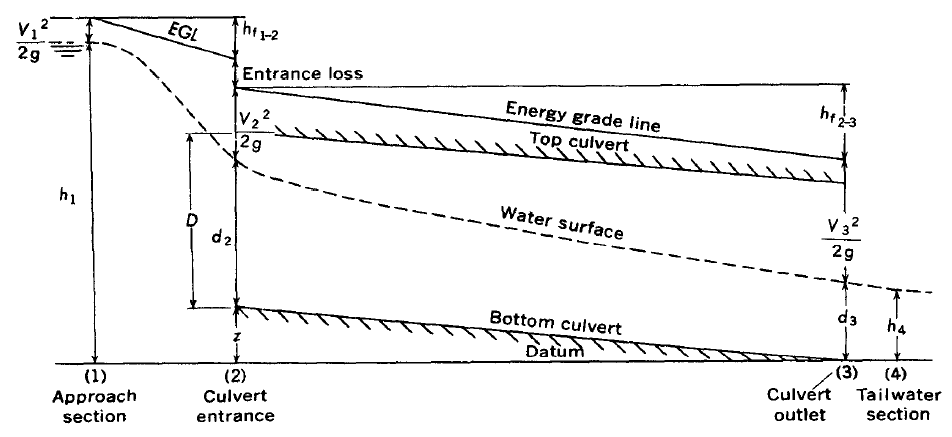
\includegraphics[width=0.95\textwidth]{culvert_fig2.png}
\end{center}
\caption{Sketch of general flow through a culvert (Bodhaine, 1968).}
\label{fig:culvert_fig2}
\end{figure}

$Z$ gives the elevation of the culvert entrance relative to the datum through the culvert exit.
The gravitational constant is given by $g$ and $h_{f12}$ is the head loss due to friction from
the approach section to the culvert entrance;
$h_{f23}$ is the head loss due to friction inside the culvert, $d_2$ and $d_3$ are the water
depths at the culvert entrance and exit, respectively;
$V_1$, $V_2$ and $V_3$ are the velocities at the approach section,
culvert entrance and culvert exit, respectively;
$D$ is the culvert height;
and $h_1$ and $h_4$ are the water depths upstream and downstream of the culvert structure.
The six types of flow classified by Bodhaine (1968) depend on the water depths
upstream and downstream of the culvert.
Figure \ref{fig:culvert_fig3} gives a schematization of the different flow types
made according to the equation for each type of flow.
The different equations are presented below.

\begin{figure}[H]
\begin{center}
  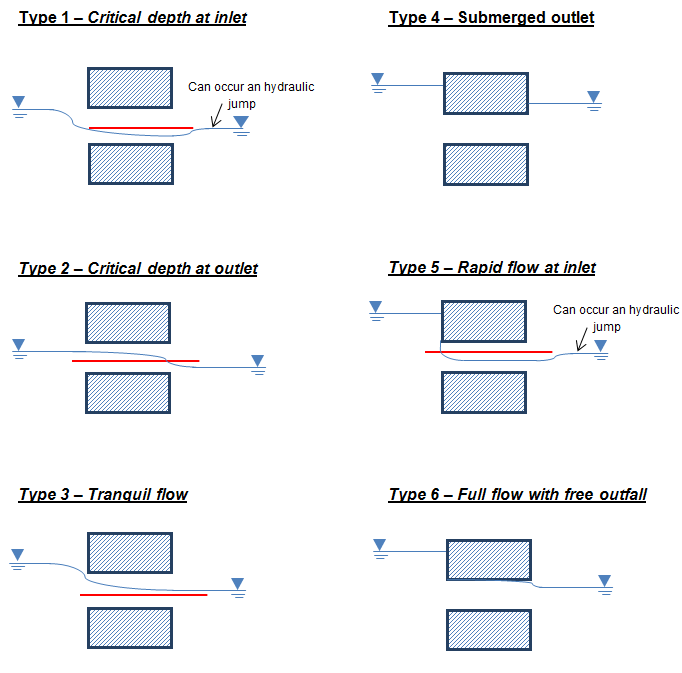
\includegraphics[width=0.7\textwidth]{culvert_fig3.png}
\end{center}
\caption{Schematization of the 6 different types of flow that occur
through culverts according to Bodhaine (1968).
The red line represents the critical water depth.}
\label{fig:culvert_fig3}
\end{figure}

\underline{\textbf{Type 1 -- Critical depth at inlet- supercritical flow at the entrance}}\\

In flow type 1 the flow is supercritical inside the culvert and the critical depth occurs
at the entrance of the culvert. The culvert slope ($S_0$) has to be greater than the
critical slope ($S_c$) and the culvert flows partially full.
For the Froude number $Fr=1$ (which is the case of flow type 1),
the discharge coefficient is typically $C_D=0.95$.
The discharge is then calculated according to the following formula:

\begin{equation}
Q = C_D A_c \sqrt{2g\left(h_1-z-h_c-h_{f12}+\alpha \dfrac{\overline{V_1}^2}{2g}\right)}
\end{equation}

with:\\
$C_D$ the discharge coefficient;\\
$A_c$ the flow area at critical water depth; \\
$g$ the gravitational constant; \\
$h_1$ the upstream water depth; \\
$z$ elevation of the culvert entrance; \\
$h_c$ the critical water depth; \\
$h_{f12}$ the head loss due to friction from the approach section to the culvert entrance; \\
$\alpha$ the kinetic energy correction coefficient for the approach section; \\
$V_1$ the average flow velocity at the approach section of the culvert.\\

\underline{\textbf{Type 2 -- Critical depth at outlet – supercritical flow at the exit}}\\

In flow type 2 the flow is tranquil inside the culvert. The critical depth is located at
the culvert outlet. The culvert flows partially full. Here the culvert slope has to be
smaller than the critical slope. The discharge coefficient is similar to flow type 1.
The discharge is then calculated according to the following formula:
\begin{equation}
Q=C_D A_c \sqrt{2g\left(h_1-h_c-h_{f12}-h_{f23}+\alpha \dfrac{\overline{V_1}^2}{2g}\right)}
\end{equation}
with:\\
$h_{f23}$ the head loss due to friction inside the culvert.\\

\underline{\textbf{Type 3 -- Tranquil flow -- subcritical flow}}\\

In flow type 3 the flow is subcritical inside the culvert. There is no critical depth.
The culvert flows partially full. Like flow types 1 and 2, the discharge coefficient
varies with respect to the Froude number, being typically between $C_D=0.82 -- 0.95$.
The discharge is calculated according to the following formula:
\begin{equation}
Q=C_D A_3 \sqrt{2g\left(h_1-d_3-h_{f12}-h_{f23}+\alpha \dfrac{\overline{V_1}^2}{2g}\right)}
\end{equation}
with:\\
$A_3$ the flow area at the culvert outlet;\\
$d_3$ the water depth at the culvert outlet.\\

\underline{\textbf{Type 4 -- Submerged inlet and outlet}}\\

In flow type 4 the culvert inlet and outlet are submerged. The culvert flows full.
The discharge coefficient varies with respect to the culvert geometry, ranging
typically between $C_D=0.75$ and $C_D=0.95$.
The discharge is calculated according to the following formula:
\begin{equation}
Q=C_D A_0 \sqrt{2g\dfrac{h_1-h_4}{1+29C_D^2 n^2 L/R^{4/3}}}
\end{equation}
with:\\
$A_0$ the flow area at the culvert entrance;\\
$h_4$ the downstream water depth;\\
$n$ the Manning coefficient;\\
$L$ the length of the culvert;\\
$R$ the hydraulic radius.\\

\underline{\textbf{Type 5 -- Rapid flow at inlet}}\\

In flow type 5, the flow is supercritical at the inlet to the culvert.
The culvert flows partially full. Type 5 flow does not usually occur.
When it does, the discharge coefficient is in general lower than the other types.
\begin{equation}
Q=C_D A_0 \sqrt{2g(h_1-z)}
\end{equation}

\underline{\textbf{Type 6 -- Full flow with free outfall}}\\

In flow type 6 the culvert flows full. The discharge coefficient is similar to the
one obtained for the flow type 4.
The discharge is calculated according to the following formula:
\begin{equation}
Q=C_D A_0 \sqrt{2g(h_1-d_3-h_{f23})}
\end{equation}
The indices of the different variables might seem a bit confusing,
but it was chosen to take the formulae from Bodhaine as they were
and not to make any changes to them.
Bodhaine differentiated between these six flow types based on conditions
given in the Table \ref{tab:culvert_tab1}.

\begin{table}[H]
\caption{Conditions for each type of flow defined by Bodhaine (1968).}\label{tab:culvert_tab1}
\begin{center}\begin{tabular}{|c|c|c|c|}
\hline
~ & $\mathbf{\dfrac{h_1-z}{D}}$ & ~ & ~\\
\hline
\textbf{Type 1} & $<1.5$    &  $\frac{h_4}{h_c} < 1.0$ & $S_0 > S_c$\\
\hline
\textbf{Type 2} & $<1.5$    &  $\frac{h_4}{h_c} > 1.0$ & $S_0 < S_c$\\
\hline
\textbf{Type 3} & $<1.5$    & $\frac{h_4}{D} \le 1.0$ & ~\\
\hline
\textbf{Type 4} & $> 1.0$   & $\frac{h_4}{D} > 1.0$ & ~\\
\hline
\textbf{Type 5} & $\ge 1.5$ & $\frac{h_4}{D} \le 1.0$ & ~\\
\hline
\textbf{Type 6} & $\ge 1.5$ & $\frac{h_4}{D} > 1.0$  & ~\\
\hline
\end{tabular}\end{center}
\end{table}

All the different culvert geometric features will affect the presence of culvert flow type 5 or 6.
To differentiate the two types, Bodhaine (1968) suggests to use the relations given in Figure \ref{fig:culvert_fig4}.
$r$ is the radius of entering rounded and $w$ is the measure of the length of a wingwall
or chamfer. First a curve corresponding to $r/D$, $w/D$ is chosen.
Then a point is set using the value for the culvert slope and for the ratio
between the culvert length and height.
If the point lies to the right of the chosen curve, the flow is type 6,
if it lies to the left of the curve, the flow is type 5.

\begin{figure}[H]
\begin{center}
  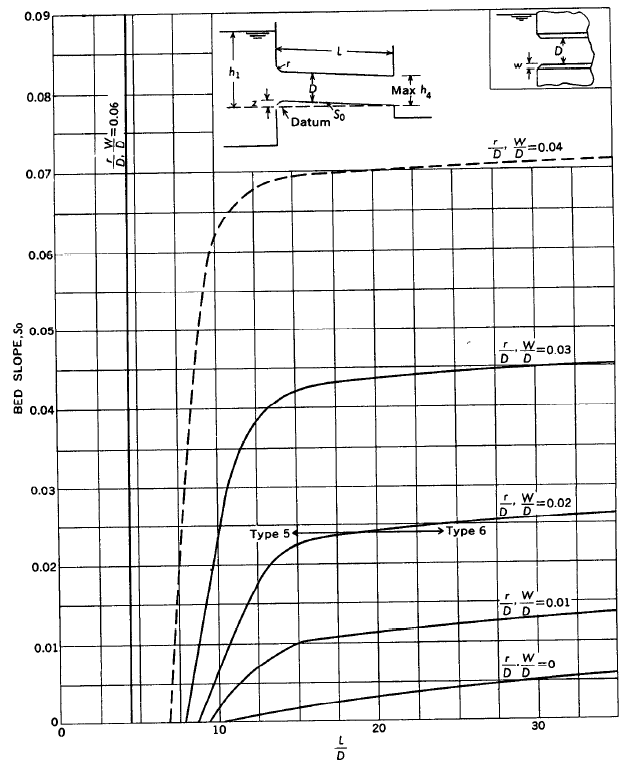
\includegraphics[width=0.6\textwidth]{culvert_fig4.png}
\end{center}
\caption{Criterion for classifying flow types 5 and 6 in concrete box or pipe culverts
with square, rounded, or bevelled entrances, either with or without wingwalls (Bodhaine, 1968).}
\label{fig:culvert_fig4}
\end{figure}

The head loss coefficients are subject of different studies made in laboratory experiments.
A number of authors have arrived to different values or empirical relationships for the
head loss coefficients. For instance, Bodhaine (1968) suggests different values for
the discharge coefficient ($C_D$) for each type of flow and depending on a number of
geometric features from the culvert. The discharge coefficients can vary from 0.39 to 0.98.
Another example is Carlier (1972) who proposes a non-dimensional coefficient $\mu$,
that for hydraulic structures made of only one culvert can be written as follows:
\begin{equation}
\mu = \dfrac{1}{\sqrt{C_1+C_2+C_3}}
\end{equation}
with:\\
$C_1$ the head loss coefficient at the entrance of the hydraulic structure;\\
$C_2$ the head loss coefficient in the hydraulic structure;\\
$C_3$ the head loss coefficient at the exit of the hydraulic structure.

If the general expression for the discharge $Q=\mu A \sqrt{2g\Delta H}$ proposed by
Carlier (1972) is compared with the formulae given by Bodhaine (1968),
it can be seen that the non-dimensional head loss coefficient ($\mu$),
incorporates both the effect of the discharge coefficient ($C_D$) and the continuous
and local head losses. $\Delta H$ is the head loss for each type of flow.

\section{Formulations for culvert simulation in TELEMAC}

TELEMAC-2D and 3D give the possibility of modelling hydraulic structures, such as bridges,
discharges under a dike or tubes in which free-surface or pressurized flows may
occur during the total simulation time.
This is done by a couple of points between which flow may occur with respect to
the water levels in the river and in the floodplain.
The subroutine BUSE is called to model this kind of structures.
Each kind of flow has its own type of discharge calculation.
The kind of formulation used to compute the flow rates can be chosen with the keyword OPTBUSE.

\subsection{Option 1 -- following Carlier's formulation}

With this first option, the different equations implemented to calculate the
discharges are dependent on the flow regime and follow Carlier (1972).
Then the velocities are deduced from the discharges and are taken into account as source
terms both in the continuity and momentum equations.
The critical water depth ($h_c$) is approximated to $h_c \approx 2/3 h_1$ (Carlier, 1972).
Figure \ref{fig:culvert_fig5} presents the different variables used to calculate the discharges.
$S_1$ and $S_2$ are the upstream and downstream water elevations, respectively, $z_1$ and $z_2$
the upstream and downstream culvert bottom elevations, $D$ the culvert height and $h_1=S_1-z_1$
and $h_2=S_2-z_2$ the upstream and downstream water depths, respectively.

\begin{figure}[H]
\begin{center}
  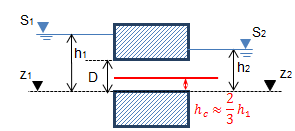
\includegraphics[width=0.5\textwidth]{culvert_fig5.png}
\end{center}
\caption{Representation of the different variables used to calculate
the discharges for each type of flow.}
\label{fig:culvert_fig5}
\end{figure}

The equations coded with this first option are described below.
Between brackets the corresponding flow type according to Bodhaine (1968) is given.
\begin{itemize}
\item Free surface flow equations:
  \begin{itemize}
  \item Submerged weir (Bodhaine type 3)
    \begin{equation}
      Q=\mu (S_2-z_2) W \sqrt{2g(S_1-S_2 )} = (S_2-z_2) W \sqrt{\dfrac{2g(S_1-S_2)}{C_1+C_2+C_3}}
    \end{equation}
  \item Unsubmerged weir(Bodhaine type 2)
    \begin{equation}
      Q=0.385 W \sqrt{2g}(S_1-z_1)^{3/2}
    \end{equation}
  \end{itemize}
\item Pressurised flow equations:
  \begin{itemize}
  \item Submerged orifice law (Bodhaine type 4)
    \begin{equation}
      Q=\mu D W \sqrt{2g(S_1-S_2 )} = D W \sqrt{\dfrac{2g(S_1-S_2)}{C_1+C_2+C_3}}
    \end{equation}
  \item Unsubmerged orifice law
    \begin{equation}
    Q= \mu D W \sqrt{2g(S_1-S_2)} = D W \sqrt{\dfrac{2g(S_1-S_2)}{C_1+C_2}}
    \end{equation}
  \end{itemize}
\end{itemize}

The user has the possibility of assigning different values for $C_1$, $C_2$ and $C_3$.
The flow direction is imposed, \textit{e.g.}, the user can specify if the flow is going
in only one direction or in both directions and in which direction.
The keyword CLP specifies this behaviour.\\
CLP=0, flow is allowed in both directions;\\
CLP=1, flow is only allowed from section 1 to section 2\\
CLP=2, flow is only allowed from section 2 to section 1\\
CLP=3, no flow allowed.\\
A relaxation parameter ($\theta$) is introduced so that the discharge is calculated
in an explicit, implicit, or semi-implicit way.
If $\theta=1$ the calculation of the discharge is explicit while if $\theta=0$
the discharge calculation is implicit:
\begin{equation}
  Q^n=\theta Q^n + (1-\theta) Q^{n-1}
\end{equation}
Relaxation gives slower convergence speed to get the final solution
but smoothes some instabilities.
If the solution does not converge because of instabilities, the coefficient can be lowered.

\subsection{Option 1 -- following Bodhaine's formulation}

With this option the discharges are calculated based on the equations proposed in Bodhaine (1968)
and similar to the ones incorporated in DELFT 3D model.
The flow type 1 conditions were not incorporated since they only
occur when the culvert slope is larger than the critical flow slope.
This only happens in very rare occasions if the culvert slope is very steep.
The equations used to compute the discharges are given below.\\

\underline{\textbf{Type 2 -- Critical depth at outlet}}\\
\begin{equation}
Q = \mu h_c W \sqrt{2g(S_1-(z_2+h_c))}
\end{equation}
with:
\begin{equation}
\mu = C_{D1}/\sqrt{1+\left[\dfrac{2gLn^2}{R^{4/3}} +C_v\right] C_{D1}^2 \dfrac{h_c}{h_s}^2}
\end{equation}
\begin{equation}
h_s=0.5h_c+0.5(S_1-z)
\end{equation}
\begin{equation}
R=\dfrac{h_s W}{2h_s+W}
\end{equation}

\underline{\textbf{Type 3 -- Tranquil flow}}\\
\begin{equation}
Q=\mu (S_2-z_2)W\sqrt{2g(S_1-S_2 )}
\end{equation}
with:
\begin{equation}
\mu = C_{D1}/\sqrt{ 1+\left[\dfrac{2gLn^2}{R^{4/3}} +C_v \right] C_{D1}^2 \left(\dfrac{S_2-z_2}{h_s}\right)^2}
\end{equation}
\begin{equation}
h_s=0.5(S_1-z)+0.5(S_2-z)
\end{equation}
\begin{equation}
  R=\dfrac{h_sW}{2h_s+W}
\end{equation}

\underline{\textbf{Type 4 -- Submerged outlet}}\\
\begin{equation}
Q =\mu D W \sqrt{2g(S_1-S_2)}
\end{equation}
with:
\begin{equation}
\mu = C_{D2}/\sqrt{1+\left[\dfrac{2gLn^2}{R^{4/3}} +C_v \right] C_{D2}^2}
\end{equation}
\begin{equation}
h_s=D
\end{equation}
\begin{equation}
R=\dfrac{h_s W}{2h_s+2W}
\end{equation}

\underline{\textbf{Type 5 -- Rapid flow at inlet}}\\
\begin{equation}
Q= \mu D W \sqrt{2gh_1}
\end{equation}
with:
\begin{equation}
\mu = C_{D3}
\end{equation}
\begin{equation}
h_s = D
\end{equation}
\begin{equation}
R = \dfrac{h_s W}{2h_s+2W}
\end{equation}

\underline{\textbf{Type 6 -- Full flow with free outfall}}\\
\begin{equation}
Q = \mu D W \sqrt{2g(S_1-(z_2+D))}
\end{equation}
with:
\begin{equation}
\mu = C_{D2}/\sqrt{1+\left[\dfrac{2gLn^2}{R^{4/3}} +C_v \right] C_{D2}^2}
\end{equation}
\begin{equation}
h_s=D
\end{equation}
\begin{equation}
R=\dfrac{h_s W}{2h_s+2W}
\end{equation}
The head loss coefficient expressions were obtained from experimental studies made at
Flanders Hydraulic Research.
The discharge coefficient, $C_D$, is dependent of each type of flow, being the same for
types 1, 2 and 3 ($C_{D1}$), then for types 4 and 6 ($C_{D2}$) and finally for type 5 ($C_{D3}$).
The conditions at which a certain type of flow occurs,
are presented in Table \ref{tab:culverts_tab2}.

\begin{table}[H]
\caption{Conditions for each type of flow used in TELEMAC with OPTBUSE = 2.}
\label{tab:culvert_tab2}
\begin{center}\begin{tabular}{|c|c|c|c|c|}
\hline
~ & $\mathbf{\dfrac{S_1-z_1}{D}}$ & $\mathbf{\dfrac{S_2-z_2}{D}}$ & $\mathbf{S_2-z_2}$ & $L/D$ \\
\hline
\textbf{Type 2} & $<1.5$    &  ~ & $< h_c$ & ~ \\
\hline
\textbf{Type 3} & $<1.5$    & $\le 1.0$ & $> h_c$ & ~\\
\hline
\textbf{Type 4} & $> 1.0$   & $> 1.0$ & ~ & ~\\
\hline
\textbf{Type 5} & $\ge 1.5$ & $\le 1.0$ & ~ & $< h_c$\\
\hline
\textbf{Type 6} & $\ge 1.5$ & $\le 1.0$  & ~ & $\ge h_c$\\
\hline
\end{tabular}\end{center}
\end{table}

The equations presented above are written to describe flow conditions through a
culvert system with a single pipe.
Nevertheless, additional features are sometimes incorporated in the hydraulic structures,
such as weirs in the vicinity of the culvert entrance or exit.
Such combined structures have to be taken into account.
Then the geometric features of the culvert presented in Figure \ref{fig:culvert_fig5}
are modified (Figure \ref{fig:culvert_fig6}).
It was decided that an equivalent culvert bottom elevation should be used,
which replaces both the bottom elevations $z_1$ and $z_2$ in the formulae decribed above.
The equivalent bottom culvert elevation is then equal to the mean between $z_1$ and $z_2$.
The diameter used in the equations will be the one corresponding to the entrance of the culvert,
\textit{i.e.}, regarding Figure \ref{fig:culvert_fig6}, if the flow goes from left
to the right $D$ will be replaced by $D_1$ and on the opposite direction,
the value $D_2$ will be used.

\begin{figure}[H]
\begin{center}
  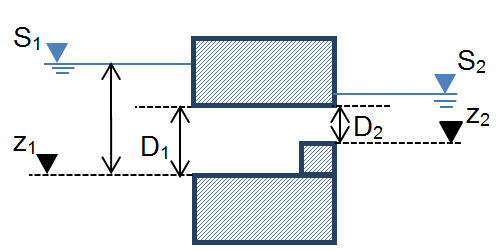
\includegraphics[width=0.5\textwidth]{culvert_fig6.png}
\end{center}
\caption{Representation of the different variables used to
calculate the discharges for each type of flow.}
\label{fig:culvert_fig6}
\end{figure}

The head loss coefficient ($\mu$ was adapted from the one calculated with the first option,
based on Carlier (1972) and is used as main head loss coefficient).
Structures that caused additional head loss, like valves, grilles (trash screens) or pilars
were added in the calculation of this main coefficient.
In this way these additional features that can be present in culvert structures of
different geometric configurations are taken into account and contribute to
the flexibility of the implementation of many types of culvert structures.
The head loss due to singularities can be obtained by the general
relation (Lencastre, 1961 and Carlier, 1972):
\begin{equation}
\Delta H = C \dfrac{U^2}{2g} ~\text{or}~  U = \mu \sqrt{2g\Delta H}
\end{equation}
with:
\begin{equation}
\mu =\dfrac{1}{\sqrt{C}}
\end{equation}

The coefficient $C$ represents the sum of the different contributions for the
head loss due to singularities:
\begin{equation}
C=C_1+C_p+C_2+C_3+C_v+C_T
\end{equation}
The different contributions to this head loss coefficient $C$ will be discussed
separately and in detail here below.\\

\textbf{Coefficient} $\mathbf{C_1}$ \\
$C_1$ represents the head loss due to the contraction of the flow at the entrance
of the hydraulic structure.
Usually it is equal to 0.5 (Figure \ref{fig:culvert_fig7}).
Usually, there is an abrupt contraction that will cause a head loss due to
the decelaration of the flow immediately after the culvert entrance.

\begin{figure}[H]
\begin{center}
  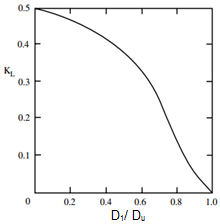
\includegraphics[width=0.5\textwidth]{culvert_fig7.png}
\end{center}
\caption{Local loss coefficient for a sudden contraction as
a function of diameter ratio between the diameter after the contraction ($D_1$)
and before the contraction $D_u$ (Bruce et al., 2000).}
\label{fig:culvert_fig7}
\end{figure}

Already in the past, Bodhaine (1968) noticed that the discharge coefficient ($C_D$)
for type 5 flow had to be lowered comparetively with the other flow types.
It seems that the calculated discharge tends to be overestimated when the
default equation is applied. In order to take into account that effect,
a correction coefficient ($\alpha_1^5$) is applied to $C_1$ when type 5 flow occurs, such that:
\begin{equation}
\Delta H_{1.5}=\alpha_1^5 C_1  \dfrac{U^2}{2g}
\end{equation}
Comparing with the values proposed by Bodhaine (1968), $4 \le \alpha_1^5 \le 10$.\\

\textbf{Coefficient} $\mathbf{C_p}$\\
Sometimes at the entrance of culverts the flow is divided into two sections
caused by two entrance boxes instead of one but than the flow converges into
a single culvert pipe. In other words a kind of pilar is dividing the flow at the entrance.
This causes additional head loss and is taken into account.
Following Carlier (1972) the head loss through parallel pillars is given by:
\begin{equation}
\Delta H_p = C_p \dfrac{U^2}{2g}
\end{equation}
where $C_p=\beta \left(\dfrac{Lp}{b}\right)^{4/3} \text{sin} \theta$  represents the head
loss coefficient due to the presence of pillars. $Lp$ is the thickness of the pillars, $b$
the free thickness between two consecutive pillars and $\beta$
a coefficient dependent on cross-shore section of the pillar.\\

\textbf{Coefficient} $\mathbf{C_2}$\\
$C_2$ represents the head loss coefficient due to the friction in the structure
and is expressed by (Lencastre, 1972):
\begin{equation}
\Delta H_2 = C_2  \dfrac{U^2}{2g} = \dfrac{2gLn^2}{R^{4/3}}\dfrac{U^2}{2g}
\end{equation}
where $L$ is the length of the structure, $n$ the Manning Strickler coefficient
of the structure and $R$ the wet cross-shore section in the structure calculated
in the code for each type of flow.
Table \ref{tab:culvert_tab3} presents the expressions for the calculation of $R$,
following what was done in the DELFT 3D model.
Here an assumption is made when calculating the hydraulic radius since the
code does not make any kind of backwater analysis to get the
precise water depths that occur in the culvert (like Mike 11 does).
\begin{table}[H]
\caption{Different parameters for each type of flow to calculate the hydraulic radius in TELEMAC-3D.}
\label{tab:culvert_tab3}
\begin{center}\begin{tabular}{|c|c|c|}
\hline
\textbf{Type of flow} & $\mathbf{h_s}$ & $\mathbf{R}$ \\
\hline
\textbf{Type 2} & $0.5 h_c + 0.5(S_1-z)$    & $R = \dfrac{h_s W}{2 h_s+W}$ \\
\hline
\textbf{Type 3} & $0.5 (S_1 - z_1) + 0.5(S_2-z_2)$    & $R = \dfrac{h_s W}{2 h_s+W}$ \\
\hline
\textbf{Type 4} & $D$    & $R = \dfrac{h_s W}{2 h_s+2W}$ \\
\hline
\textbf{Type 5} & $D$    & $R = \dfrac{h_s W}{2 h_s+2W}$ \\
\hline
\textbf{Type 6} & $D$    & $R = \dfrac{h_s W}{2 h_s+2W}$ \\
\hline
\end{tabular}\end{center}
\end{table}

\textbf{Coefficient} $\mathbf{C_3}$\\
$C_3$ is the head loss coefficient due to expansion of the flow exiting the culvert.
It can be given by (Lencastre, 1961):
\begin{equation}
\Delta H_3 = \left(1-\dfrac{A_s}{A_{s2}}\right)^2 \dfrac{U^2}{2g} = C_3\dfrac{U^2}{2g}
\end{equation}
where $A_s$ and $A_{s2}$ are the sections in and at the downstream part of the structure.
Usually is equal to the unity for a sudden enlargement.\\

\textbf{Coefficient} $\mathbf{C_V}$\\
$C_V$ is the head loss coefficient due to the presence of a valve.
The head loss due to valves ($\Delta H_v$) can also be estimated:
\begin{equation}
\Delta H_v = C_V\dfrac{U^2}{2g}
\end{equation}
where $C_V$ depends on the type of valve and the degree of opening.
For a gate valve, some values were obtained experimentally,
and they depend on the opening of the valve (Bruce et al., 2000):
see Table \ref{tab:culvert_tab4}.
\begin{table}[H]
\caption{Values for the head loss coefficient depending on the opening of a gate valve.}
\label{tab:culvert_tab3}
\begin{center}\begin{tabular}{|c|c|}
\hline
~ & $C_V$ \\
\hline
\textbf{Wide open} & 0.2\\
\hline
\textbf{3/4 open} & 1.0 \\
\hline
\textbf{1/2 open} & 5.6 \\
\hline
\textbf{1/4 open} & 17 \\
\hline
\end{tabular}\end{center}
\end{table}

Again, a correction coefficient ($\alpha_v^5$) is applied to the head loss coefficient
due to a valve in order to take into account the increase of the head loss when type 5
flow occurs (Eq. 4.12).
Through a number of laboratory experiences (IMDC Report 613\_9\_1), it can be seen that when
type 5 flow occurs, there is a greater influence of having a valve:
the associated head loss coefficient is in general much higher than for the other types of
flow (Figure  \ref{fig:culvert_fig8}).
Please note that the variable $\alpha$ in Figure \ref{fig:culvert_fig8}
is not the same as $\alpha_v^5$.
Figure \ref{fig:culvert_fig8} is given here just to show the influence of
the valve in the different types of flow.
\begin{equation}
\Delta H_{v5} = \alpha_v^5 C_v \dfrac{U^2}{2g}
\end{equation}

\begin{figure}[H]
\begin{center}
  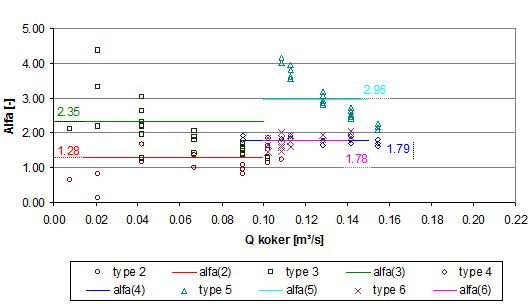
\includegraphics[width=0.95\textwidth]{culvert_fig8.png}
\end{center}
\caption{Discharge coefficient (Alfa) due to the presence of open valves for
each type of flow (source: IMDC Report 613\_9\_1)}
\label{fig:culvert_fig8}
\end{figure}

\textbf{Coefficient} $\mathbf{C_t}$\\

Trash screens are usually present at the inlet of culverts to prevent garbage
from entering or blocking the culvert. The head loss due to trash screens
($\Delta H_t$) can be estimated by its relationship with the velocity
head through the net flow area.
A number of expressions were obtained in the past by several authors.
We use the expression given by the Bureau of Reclamation (1987):
\begin{equation}
\Delta H_t = (1.45-0.45A_t-A_t^2)\dfrac{U^2}{2g} = C_t \dfrac{U^2}{2g}
\end{equation}
where $A_t=\frac{Anet}{Agross}$ gives the ratio of net flow area to gross rack area.
$U$ is the net flow velocity. The value for $C_t$ can vary between $C_t= 0$ equivalent
to not having any trash screens to approximately $C_t= 1.4$, for which the net
flow area is almost equal to the gross rack area.

Note that a very similar fomulation to this second option is included in DELFT 3D.
The main difference between the second culvert functionality in TELEMAC and the one
included in DELFT 3D is the way how the head loss coefficient is calculated.
While in TELEMAC, the Carlier (1972) reference was followed, in DELFT 3D they refer
to experiments executed by Flanders Hydraulic Research.


\subsection{Transport of tracers through culverts}


With the implementation of the culvert functionality,
some modifications had to be done in the code such that
it would be possible to model the passage of the tracer through the culvert structure.
Following the same idea implemented to model the flow through culverts,
the concentration of the tracer in the model domain is assigned to source and sink terms
for tracers. When the flow goes from the river to the floodplain,
there is a source point in the floodplain with a tracer concentration equal to the one
in the river. At the same time in the river there is a sink term with the same tracer
concentration. The opposite happens when the flow goes from the floodplain to the river.
Please note that it is the tracer concentration that is assigned to the source term
and not the tracer concentration per second.
In its structure, TELEMAC deals with that concentration and associates it to the
discharge and volume of fluid at the source terms.
In order to take into account the transport of tracers in the model the
user has only to specify in the steering file the keywords relative to the tracers.

\section{TELEMAC input files and the implemented code}

In order to take culverts into account in TELEMAC the user has to define in the
steering file two keywords: \\
NUMBER OF CULVERTS \\
CULVERTS DATA FILE\\

The number of culverts has to be assigned to the keyword NUMBER OF CULVERTS
(please note that this is the number of culverts and not the number of sources/sink terms:
one culvert has two sink/source terms).
The keyword CULVERTS DATA FILE refers to an ASCII file where the geometric characteristics
and all head loss coefficients are given to be used by the code.
The text file has to follow a strict structure of the input parameters in order
for the software to read the right values for the right parameter.
Here below an example is given:\\

Relaxation, Number of culverts\\
0.05 2\\
I1  I2  CE1  CE2  CS1  CS2  LRG HAUT1 CLP LBUS Z1 Z2 CV  C56  CV5  C5 CT HAUT2 FRIC LENGTH CIRC\\
data culvert 1  ...\\
data culvert 2 ...\\
... \\

The index number 1 refers to the river side and the index 2 refers to the floodplain side.
I1 and I2 correspond to the index of the source/sink terms in the river side
and in the floodplain that represent the beginning and end of the culvert.
CE1, CE2 and CS1, CS2 are the head loss coefficients
for the inlet and outlet sluice entrance ($C_1$) and exit ($C_3$), respectively.
LRG represents the width of the culvert.
HAUT1 and HAUT2 the height of the culvert at the river and
floodplain side.
The flow direction is also imposed through the keyword CLP and
a relaxation parameter (variable RELAXB) is incorporated in the code.
LBUS is the linear head loss in the culvert.
Z1 and Z2 the elevations of the culvert
extremities in the river side and in the floodplain.
CV refers to the loss coefficient due to the presence of a valve ($C_v$) and
C56 ($c$) is the constant used to differentiate flow types 5 and 6.
C5 and CV5 represent correction coefficients to C1 and to CV coefficients
due to the occurrence of the type 5 flow.
CT is the loss coefficient due to the presence of trash screens ($C_t$).
FRIC is the Manning Strikler coefficient.
The length of the culvert can be set (LENGTH parameter), and its shape can be specified through the parameter CIRC (equal to 1 in
case of a circular section, 0 for a rectangular section).



